\documentclass{article}

% if you need to pass options to natbib, use, e.g.:
%     \PassOptionsToPackage{numbers, compress}{natbib}
% before loading neurips_2018

% ready for submission
%\usepackage{nips_2018}

% to compile a preprint version, e.g., for submission to arXiv, add add the
% [preprint] option:
\usepackage[preprint]{nips_2018}

% to compile a camera-ready version, add the [final] option, e.g.:
%\usepackage[final]{nips_2018}

% to avoid loading the natbib package, add option nonatbib:
%\usepackage[nonatbib]{nips_2018}

\usepackage[utf8]{inputenc} % allow utf-8 input
\usepackage[T1]{fontenc}    % use 8-bit T1 fonts
\usepackage{hyperref}       % hyperlinks
\usepackage{url}            % simple URL typesetting
\usepackage{booktabs}       % professional-quality tables
\usepackage{amsfonts}       % blackboard math symbols
\usepackage{nicefrac}       % compact symbols for 1/2, etc.
\usepackage{microtype}      % microtypography
\usepackage{graphicx}

\title{Random Network Distilation for Out-of-Distribution detection}

\begin{document}
% \nipsfinalcopy is no longer used

% Recomendations:
% 1) The figure number and caption always appear after the figure. Place one line space before the figure caption and one line space after the figure. The figure caption should be lower case (except for first word and proper nouns); figures are numbered consecutively.
% 2) The table number and title always appear before the table. Place one line space before the table title, one line space after the table title, and one line space after the table. The table title must be lower case (except for first word and proper nouns)
% 3) Note that publication-quality tables do not contain vertical rules.

\maketitle

\begin{abstract}
    This paper represents a review on the paper \cite{pitfalls} along with my analysis of the problem of Out-of-Distribution (OoD) detection. While \cite{pitfalls} presents broad analysis of in-domain uncertainty and proposes a technique that increases quality of in-domain uncertainty estimation, I provide analysis and overview of common approaches for a complimentary task of OoD detection and finally come up with a new approach that apparently can improve quality of OoD detection in Neural Machine Translation (NMT).
\end{abstract}

\section{Introduction}
    In a wide range of tasks deep neural networks achieve state-of-the-art performance. However, there is a bunch of applications like autonomous vehicles, where their deployment is limited now because of their inability of being uncertain when they are wrong. There are two different sources of errors: interpolation error and extrapolation error. Interpolation error usually occurs on in-domain samples and it's caused by noisy training data and imperfection of a neural network architecture. Extrapolation errors come when the net is trying to make a prediction for an Out-of-Distribution (OoD) sample. In both of these scenarios a neural net can be very certain in its prediction yet being wrong. A lot of approaches were proposed to address uncertainty estimation. \cite{pitfalls} focuses on in-domain uncertainty and in my further analysis I'll be focusing on Out-of-Distribution uncertainty and methods of OoD detection.

\section{Paper review}
\subsection{Ensembles of neural networks}
    Ensemble-based methods achieve state-of-the-art performance in both in-domain and Out-of-Distribution uncertainty quantification for almost all deep learning applications. They accomplish it by summarizing predictions of different models. A straightforward way to improve quality of in-domain uncertainty estimation is to improve ensembling techniques. The method called Deep Ensembles \cite{ensembles} shows better performance then its competitors for the same amount of members in an ensemble. The paper \cite{pitfalls} provides a nice overview of a wide range of ensembling techniques and analyzes their strengths and weaknesses. Then the authors propose a framework for their unified comparison called Deep Ensemble Equivalent score (DEE), which is basically a number of independently trained networks in the Deep Ensembles method that achieve the same quality as a considered ensemble. The value can also be non-integer, it this case it's linearly interpolated. The score itself doesn't have much value. What has value is that the authors showed using this score that many of popular ensembling techniques are very resource-wasting, because they're equivalent to deep ensembles with just a few members.

\subsection{Metrics for in-domain uncertainty quantification}
    There're several commonly used metrics that asses quality of in-domain uncertainty quantification like average test log-likelihood, Brier score, misclassification detection and others. The authors show that most of these commonly used metrics are incorrect and don't meet simple and reasonable requirements, which authors propose themselves. For instance they state it's incorrect to compare non-calibrated models using just a log-likelihood, because this may lead to an arbitrary ranking of methods and only calibrated scores are allowed. In fact it was showed many times for many different deep learning applications that model calibration improves quality of the main task or doesn't affect it in some cases. So here the authors proved that it's not the case where the quality isn't affected. They stopped on the idea of using calibrated log-likelihood score as the ideal metric to estimate in-domain uncertainty, which also correlates well with total error of an ensemble on its original task.

\subsection{Test-time-augmentation}
    The most important contribution of the paper from my point of view is that the authors combined test-time-augmentation with ensembling. They proposed to feed different augmented objects into different networks from an ensemble. This trick inproved quality of in-domain uncertainty estimation. While the trick seems quite easy to invent I haven't heard of that from papers earlier. The only trouble is that it's not practical to use ensembles directly, while they can be distilled \cite{end2}. And it's not obvious how to distil an ensemble that takes different augmented objects as inputs into a single network and run its inference just a single time. I was thinking on this question and came up with no idea.

\subsection{Overall evaluation}
    The paper is easy to read and well structured. The authors made a broad overview of popular methods and provided reasonable analysis. The code is available. The only weak point I can find here is that the results are not a breakthrough and the ideas are not something anyone never thought before (like the transformer architecture \cite{transformer} or Neural ODE). At the same time I think it's a good paper, its main advantage is that it summarizes knowledge, which researches would otherwise need to collect themselves from different sources and the provided analysis helps avoid mistakes, which are too easy to make without it.

\section{Popular methods for OoD detection}
    In this section I'd like to review some popular methods for OoD detection, to show their advantages and drawbacks which will be used to analyze properties and areas of application of the new method, which I'd like to propose in one of the later section. For the sake of concreteness I choosed to limit reasoning with the problem of OoD detection in classification tasks. These also include sequence-to-sequence tasks like ASR and NMT. The analysis can be easily extended for the regression task as well.

\subsection{Bayesian ensembles from different points of view}
    Bayesian ensembling technique is based on a theoretical concept of obtaining a posterior distribution of model's outputs given training dataset. There shouldn't be any dependence on certain model's parameters. That's why one should compute expected value of likelihood of model's outputs taken by posterior distribution of model's parameters:

    $$p( \textrm{out} | \textrm{in}, \mathcal{D}) = \int p( \textrm{out} | \textrm{in}, \theta) p(\theta | \mathcal{D}) d \theta$$

    Then one might say that training of different randomly initialized neural nets induces an approximation for the posterior distribution $q(\theta) \approx p(\theta | \mathcal{D})$. And then the expected value can approximated by Monte-Carlo sampling.

    The entropy of the predictive posterior distribution (i.e. total uncertainty) can be decomposed into aleatoric or data uncertainty and epistemic or model uncertainty in a reasonable way:

    $$\underbrace{\mathcal{H} [ \mathbb{E}_{p(\theta | \mathcal{D})} p (\textrm{out} | \textrm{in}, \theta) ]}_{\textrm{Total uncertainty}} \,\,\,\, = \underbrace{\mathcal{I}[ \textrm{out}, \theta | \textrm{in}, \mathcal{D} ]}_{\textrm{epistemic uncertainty}} + \,\,\,\,\,\, \underbrace{\mathbb{E}_{p(\theta | \mathcal{D})} \mathcal{H} [ p(\textrm{out} | \textrm{in}, \theta) ]}_{\textrm{aleatoric uncertainty}}$$

    The aforementioned mechanism for epistemic uncertainty estimation can be viewed from a different angle. Specifically we are using an ensemble of models to estimate the extrapolation error of a single model. In some sense OoD samples are far from the training data distribution and the model does extrapolation on those samples insted of interpolation. The extrapolation problem is ill-posed, slight changes in the input data or model initialization can cause the model to learn a different function, and the difference between values of the function tend to quickly increase with increasing distance from the training set. In the case the training data is well-separable and if the right model was chosen for the task, the decision boundry should be stable in areas with high training data density. Which means the predictions on that training samples should only slightly vary as opposed to samples with low density of training data and those with OoD data specifically. Also that means the bayesian ensembles implicitly create a boundry (don't confuse with the decision boundry separating classes in the original task) that surrounds training data and separates them from the rest of the space. The Figure \ref{fig:decision_boundaries} illustrates this effect with decision boundaries that can be possibly learned by neural nets. The examples shown in the figure are imaginary and are created just to illustrate the concept. It also should be mentioned that in almost all cases we don't have an explicit access to a suitable space, where points look like in the Figure \ref{fig:decision_boundaries}. We may only assume it exists.

\begin{figure}[h]
    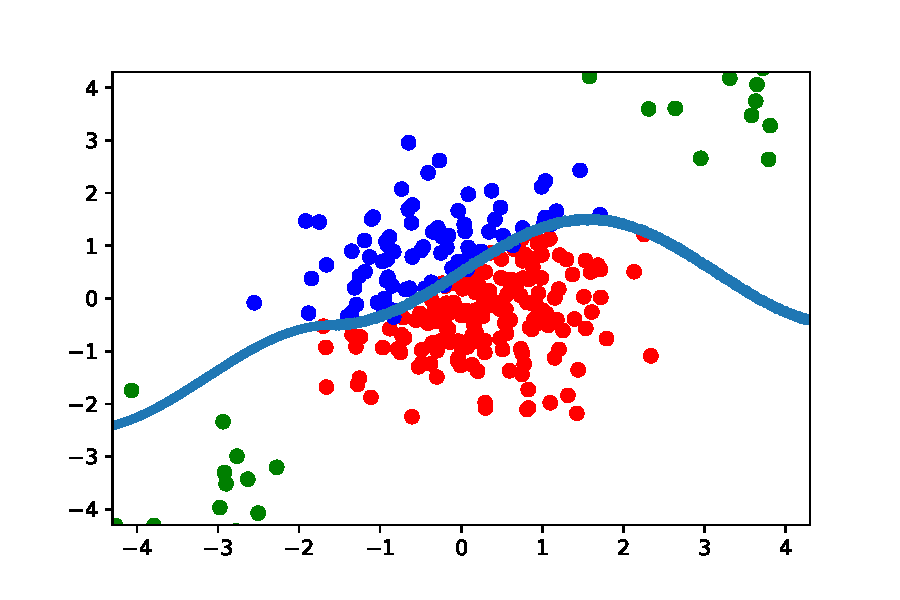
\includegraphics[scale=0.45]{samples_div_1.pdf}
    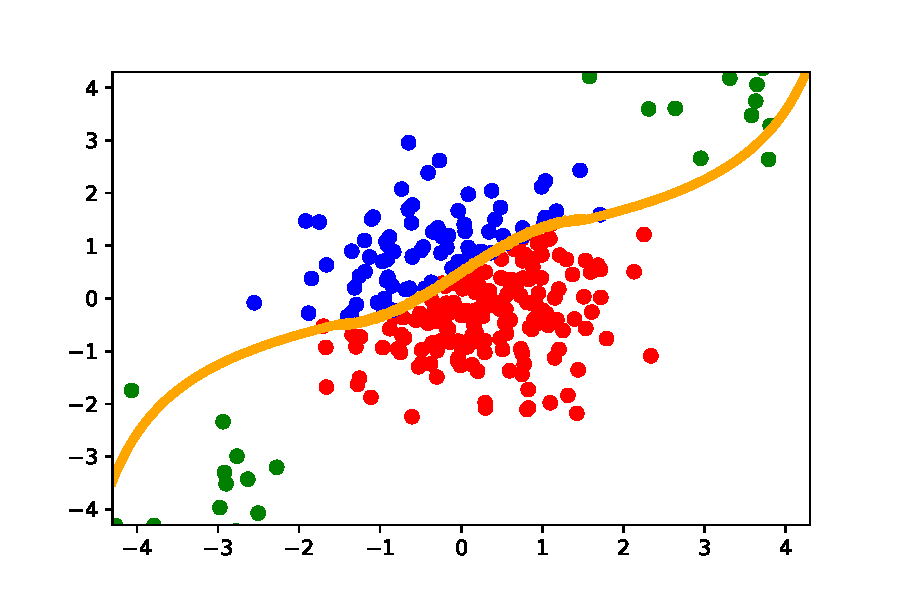
\includegraphics[scale=0.45]{samples_div_2.pdf}
    \caption{A toy example that shows how decision boundaries learned by different neural nets of an ensemble may differ in the areas which are far from the training data distribution. Red and blue points represent objects of negative and positive classes respectively and green points represent OoD samples}
    \label{fig:decision_boundaries}
\end{figure}

    Mutual information which is used for epistemic uncertainty quantification can be also be viewed as a measure of prediction variance and as a function, which can help to detect regions of extrapolation. With increasing number of diverse networks in the ensemble one can more accurately find these regions. Also as it was shown in \cite{pitfalls}, test-time-augmentation helps to achieve better in-domain uncertainty estimates. I believe it should also improve out-of-domain uncertainty estimates, because I think it increases variance of predictions in areas of extrapolation more than it increases the corresponding variance in areas of more stable decision boundary.

    There are also methods that approach the OoD detection problem by solving an additional classification problem with labeled OoD data. These approaches have limited application, because they have their own regions of in-domain and out-of-domain data.

    Bayesian ensembles don't have such a drawback. The information theoretical properties of mutual information as well as the instability property of extrapolation task, which make corresponding regions easily identifiable make ensembling methods almost universal. They show state-of-the-art performance in OoD detection on a wide range of tasks. We can even see these models obtaining 100\% ROC-AUC scores on OoD detection in ASR \cite{structured_prediction}. However, the ensemble models don't obtain 100\% scores in all scenarios of OoD detection task and sometimes perform poorly e.g. recognizing sentences from foreign language like German and French allthough the corresponding NMT model was trained to translate from English \cite{structured_prediction}. In this scenario one can expect a language model to distinguish those sentences better than on 42\% or 69\% ROC-AUC (Table 14 in \cite{structured_prediction}).

\subsection{Label-free models}
    Now let's consider models that don't require labeling. These are generative models and some reconstruction based models. It might seem these models should perform worse than ensembles of discriminative models, because they don't take into account some important information, which can be extracted from labels of objects, but at the same time they are free from negative effects that come from a learning task on noisy labels and farmful inductive biases of discriminative models.

\subsubsection{Reconstruction based models}
    The most famous representative of this family of models is the autoencoder. The idea behind reconstruction based models is that these models are expected to work better on the data they've seen during training and on objects similar to those than on OoD objects. Thus their good score on objects may be treated as the evidence of some similarity with training objects. The assumption sounds reasonably, but is wrong \cite{autoencoders}. Some objects due to their simple structure can achieve lower error values, being OoD at the same time. In the experiments later I show the poor performance of autoencoders. Although this method is not widely used due to it's poor performance, the idea behind it is interesting and can be used for invention of new methods.

\subsubsection{Generative models}
    Generative models like Variational Autoencoders (VAEs) \cite{vae}, language models (LMs), PixelCNNs and normalizing flows try to model a probability density function of the training set either explicitly like normalizing flows, PixelCNNs and LMs or implicitly like VAEs. It should be mentioned that although VAEs don't provide the ability to exactly compute density of a given data point, it can be done by Monte-Carlo approximation \cite{vae}. The concept behind using these models is the following: by assigning high probability density values to training objects (and to objects similar to them), these models would assing low density to OoD objects, because the total probability mass is constant and the models try to maximize the exact likelihood of the training data (like normalizing flows and LMs) or its lower bound (like VAE).

    Almost all these models (except LMs for which I haven't found a corresponding analysis) surprisingly fail to correctly classify OoD samples assigning higher values to many of OoD data points than to points from the training set \cite{do_dont_know}. One of the explanation why this happens is that some OoD objects just happened to have smaller variance in their original space. For instance it was shown in \cite{do_dont_know} that one can increase likelihood of images by their transformation into gray-scale. This is an example of a drawback caused by the learning problem itself (i.e. its objective). Another reason that explains such bad behaviour applies to normalizing flows: there are harmful inductive biases of the network architecture. For instance RealNVP model assigns high density values to well-structured images regardless of their content \cite{norm_flows_fail}. The coupling layers of RealNVP collect information about local correlation of pixels rather than global semantic information.

\section{OoD detection in NMT}
    Let's go back to the problem of OoD detection in NMT and poor performance of ensemble-based models. I believe it's caused by an inductive bias of the transformer model \cite{transformer} trained for the machine translation task. Transformer model tends to copy unknown words instead of translating them randomly. This behaviour can be explained by training data: in many publically available datasets (including WMT) some rare words, which shouldn't be changed in their way of writing are left written the same way in translated sentences. Maybe sometimes the entire sentences are copied-through and if this is not the case of some short sentences, these are noises in the training data. It's my assumption that copy-through behaviour is caused by the following reason. Copying-through is a very straightforward way to deal with unknown tokens in an input sequence, which a transformer model was practicing during training. So now the model a priori can copy-through all the tokens and it's not making it when it has some strong knowledge about the input tokens. So the specific structure of labels and possibly some inductive biases of the transformer architecture force it to copy-through OoD sentences. This is a strong bias which prevents models from being very diverse in cases where they should be. So as I mentioned before I think this is the case, where a language model should perform better. Although even if a language model will handle the task of language definition well, there might be some other datasets, which are OoD and which a language model won't be able to detect, just like PixelCNN trained on CIFAR-10 fails to tell SVHN is OoD dataset \cite{do_dont_know}.

\section{Random Network Distilation}
    As long there wasn't found an ideal model for OoD detection in NMT, I came up with an idea of using Random Network Distilation (RND) for this task. RNDs were proposed in \cite{random_network} for novelty detection in Reinforcement Learning (RL) to obtain better exploration. The idea is the following: there two randomly initialized neural nets and one of them (teacher) is freezed. Another one is trained on the training dataset to predict teacher's outputs. On those inputs which student has never seen before and which are different from other training examples, student won't be able to predict teacher's outputs, because these outputs are irregular. Thus the error will be high. This approach is similar to using autoencoders except it shouldn't suffer from objects with easy structure. To the best of my knowledge this method wasn't used outside RL and generally didn't get much attention, although it could be used for OoD detection in all scenarios where other approaches mentioned above can be used.

    I think this idea has many of its own drawbacks and its own inductive biases and I think they should be investigated and maybe some drawbacks can be removed. Also maybe for OoD detection in NMT this method would work better than language models and ensembles of discriminative model due to potential absence of previously discussed drawbacks of the aforementioned models. Obviously all these discussions about RND approach are just hand-waving and they need to be checked either empirically or theoretically.

    I've conducted several small experiments \footnote{The code with experiments is available on \href{https://github.com/MichaelSolotky/sandbox/tree/master/Machine\_Learning/Random\_network\_distilation}{github}} to prove this model is able to work well and sometimes better than autoencoder. During experiments I noticed it's more difficult (takes more iterations for convergence with a tuned learning rate) to distill a single random neural network than to train one classification network.

    There are some well known pairs of datasets (e.g. CIFAR-10 -- SVHN, Fashion MNIST -- MNIST) with the property that if a generative network is trained on the first, it can't accurately tell that images from the second dataset are OoD \cite{do_dont_know, norm_flows_fail}. So in my experiments I distilled a small CNN on Fashion MNIST and was testing it on MNIST and vice versa. Along with the distilation I trained an autoencoder with similar architecture twice on both of the datasets and tried to test on that one didn't use for training. To measure quality of OoD detection I used ROC-AUC. As a loss function I tried to use forward and reverse KL divergence between distributions that the teacher and the student networks produce. There was no difference between forward and reverse KL by the end of the training. The eventual performance results are in the table \ref{table}. Also there training history plots In the Figures \ref{fig:learning_on_fashion} and \ref{fig:learning_on_original}.

\begin{figure}[h]
        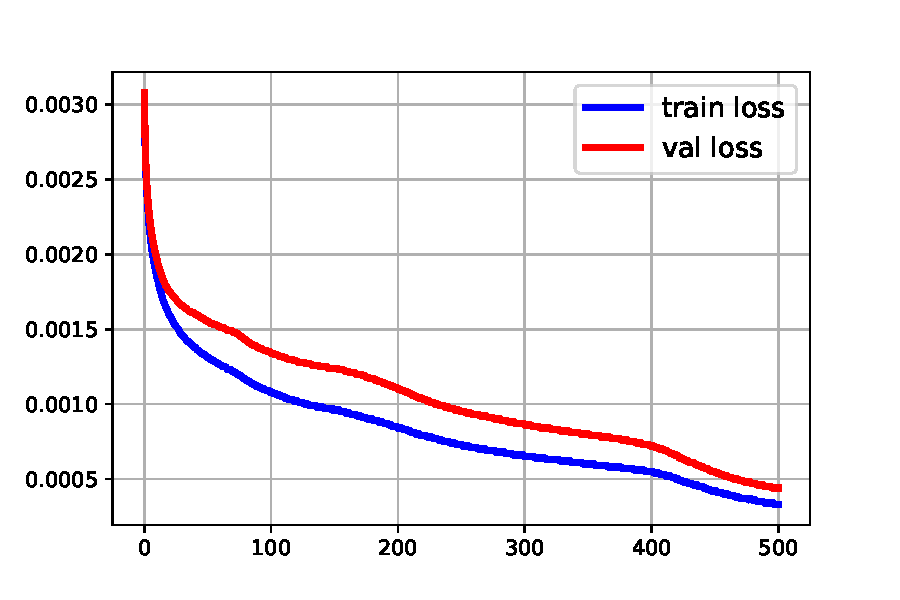
\includegraphics[scale=0.45]{learning_curves_train_fashion_to_original.pdf}
        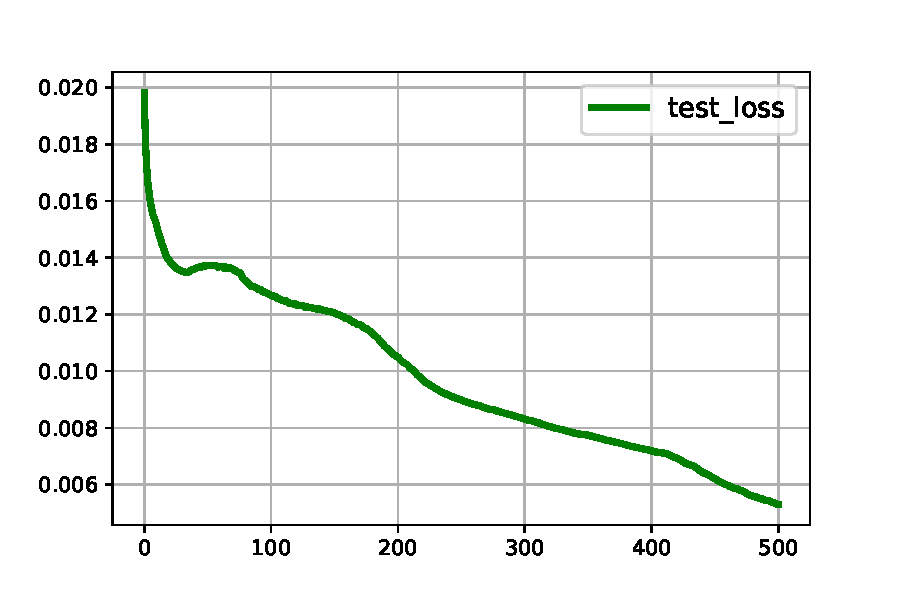
\includegraphics[scale=0.45]{learning_curves_test_fashion_to_original.pdf}
    \caption{The training history of RND on the Fashion MNIST $\rightarrow$ MNIST direction. The training was set to 500 epochs. Although the process didn't converge, the eventual performance is predictable from difference of errors on the training and testing sets and is close to ideal}
    \label{fig:learning_on_fashion}
\end{figure}

\begin{figure}[h]
    \begin{center}
        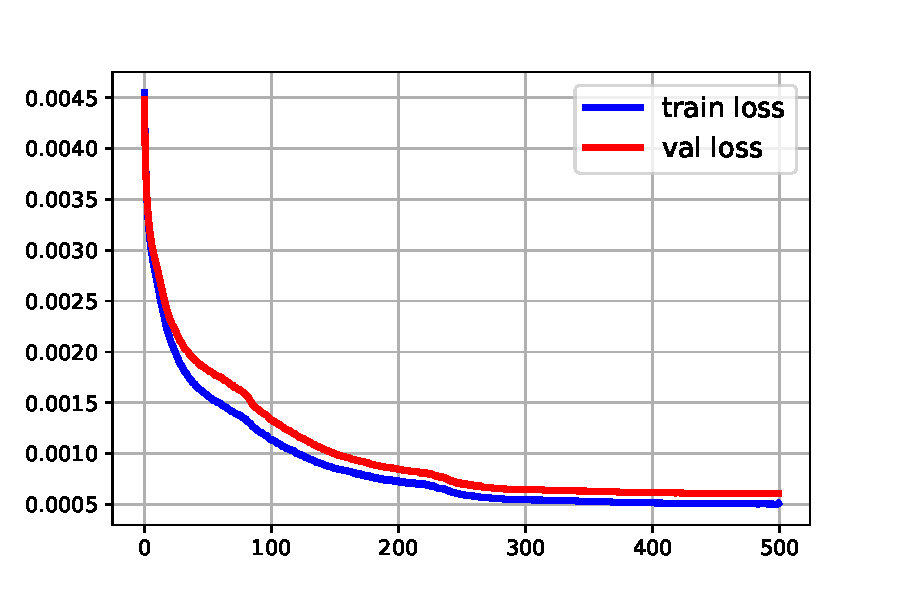
\includegraphics[scale=0.45]{learning_curves_train_original_to_fashion.pdf}
        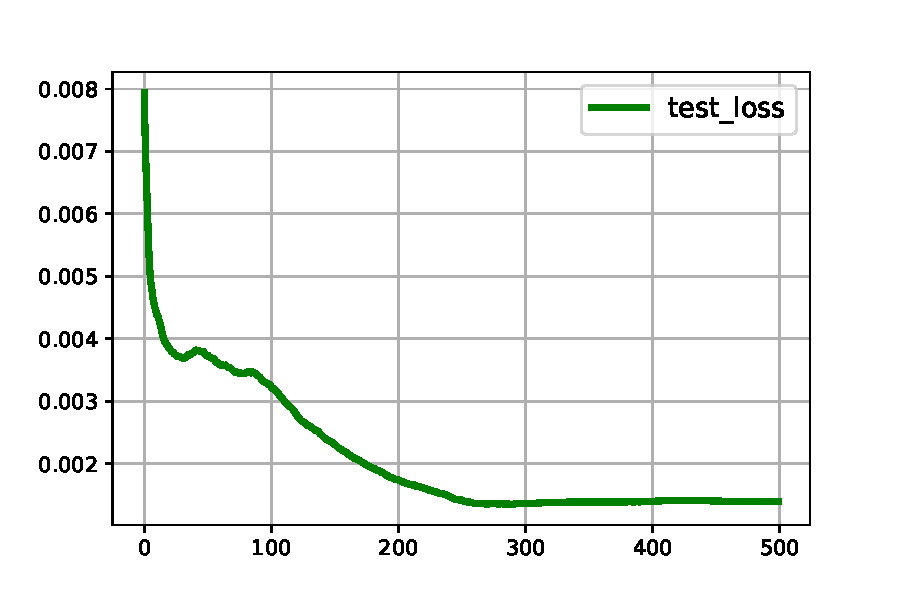
\includegraphics[scale=0.45]{learning_curves_test_original_to_fashion.pdf}
    \end{center}
    \caption{The training history of RND on the MNIST $\rightarrow$ Fashion MNIST direction}
    \label{fig:learning_on_original}
\end{figure}

\begin{table}[h]
  \caption{Comparison of detection quality of autoencoder and RND on MNIST and Fashion MNIST. It seems interesting these models show exceptional quality on different dataset pairs. We can't say one model is universally better.}
  \label{table}
  \centering
  \begin{tabular}{lll}
    \toprule
    \multicolumn{2}{r}{ROC-AUC on OoD detection}                   \\
    \cmidrule(r){2-3}
    Train $\rightarrow$ Test datasets     & RND     & Autoencoder \\
    \midrule
    Fashion MNIST $\rightarrow$ MNIST & 0.991 & 0.708      \\
    MNIST $\rightarrow$ Fashion MNIST & 0.852 & 0.997      \\
    \bottomrule
  \end{tabular}
\end{table}

\newpage
\section{Future Work}
    There are still several open questions:
    \begin{enumerate}
        \item Can the result with a small CNN on the pair MNIST -- Fashion MNIST be generalized for other dataset pairs and larger architectures?
        \item How eventual performance changes depending on starting point?
        \item Is an ensemble of distilled random networks working way better that just one random network?
        \item If the answer for the previous question is yes, can we beat ensembles of discriminative models with ensemble of distilled random networks not only in NMT scenario?
        \item What are the inductive biases of distilled random networks?
        \item Do distilled random networks truly not suffer from the drawbacks of their competitors, which were mentioned above?
    \end{enumerate}

    So to answer the first and the second questions I'm going to run training with different dataset pairs like CIFAR-10 -- CIFAR-100 or CIFAR-10 -- SVHN firstly with a small neural network. On early stage of the research I'd consider image classification task because it's relatively easy comparing to NMT or image captioning, but later I'll try many different other settings in case image classification results are satisfactory. I'm going to run the training in the same setting for a lot times (like 20 or 30 times), store the history on training, validation and test sets and also measure how the OoD detection quality changes over time. I expect eventual performance to be relatively the same on all the runs, but I think histories of performance are going to be completely different. Every single problem in this setting is unique and has it's own difficulty and number of iterations needed for convergence. Also it's still possible that some runs will finish with fail i.e. poor quality on OoD detection, against my expectations. If that happened too many times, I would need to investigate it. Also it should be checked how the eventual performance change with the size of neural network. It should be checked how batch normalization affects the stability of eventual performance results. With all different settings checked it will be clear how to come up with recommendations for random network distillation in the context of OoD detection.

    Regardless of the answers to the first two questions, ensembling makes particularly any machine learning algorithm better. There are two setting of how we can use ensembling here. First is to just average prediction error between students and teachers and the second is to use decomposition of total uncertainty into epistemic and aleatoric. Although in that case instead of measuring entropies of predictive distribution one should measure variance of error values between teacher's and student's predictions. In the end distribution of errors of such ensemble can be distilled into a single neural net in the way similar to \cite{end2}. The difference is that here the predictions are not categorical distributions, but real-valued errors.

    The fourth question requires basic comparison of performance. Nothing special here.

    The fifth question is very difficult and I'm not ready to discuss the ways of its answering right now. But the approaches to the question need to be done.

    The sixth question can be answered by simply comparing performance of distilled random networks with performance of their competitors on specially crafted data on which the drawbacks of the latter models reveal.

\section{Conclusions}
    Let's summarize: we've got a very strong mechanism based on bayesian ensembles that is able to detect regions of extrapolation. Due to harmful inductive biases of some neural net architectures, the drawbacks that come from training objectives and noises in the labels, ensembles of discriminative models tend to predict the same values in the regions, where they are supposed to act more diversly. Thus in those regions the extrapolation effect isn't detected (that's is my assumption). Distilled random networks \cite{random_network} aren't sufferring from some of the inductive biases of discriminative networks and noisy labels. Also it seems possible to avoid the drawbacks of generative and reconstruction-based models caused by their training objectives (e.g. minimization of reconstruction loss in autoencoders encourages the network to reconstruct simple images better than complex ones) using randomness of targets on OoD data. One can also use many differently initialized distilled random networks, which will probably provide different error values on OoD data. The idea of random networks can be combined then with extrapolation detection ability of bayesian ensembling technique.

\bibliographystyle{unsrt}
\bibliography{report}

\end{document}
